\chapter{Introduction}\label{C:intro}
\section{Overview}
Agile and Agile processes are used all across the world within many different software teams \hl{find stat about this}. But when it comes to using agile practices within the workplace, their is not one tool that allows you to do them online, some tools such as JIRA \cite{jira} and Trello \cite{trello} integrates parts of the agile process but not all. 

While these tools do some of the agile process, teams are still preferring physical cardwalls when it comes to doing agile processes \cite{DBLP:conf/agiledc/GossageBB15, 6005503}. In a digital age, physical cardwalls have their drawbacks in terms of not storing data in an easy accessible place and not easily integrated into distributed software teams. \cite{xp2017_aWall}. The previous tools mentioned \cite{jira,trello} do allow for online distributed teams to hold agile meetings such as Sprint Planning, but we find that they do not have a way of facilitating a agile retrospective for a distributed team. Because of this, Agile Retrospectives are still preferred to be done with physical cardwalls. 

Due to this aWall was created, it is a digital touch application that is being built as a joint software project between Victoria University of Wellington and FHNW in Switzerland between Dr Craig Anslow and Professor Martin Kropp.

\begin{figure}[ht]
\centering
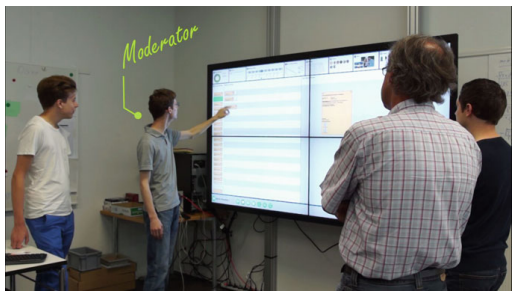
\includegraphics[width=0.85\columnwidth]{aWall_introduction}
\caption{Project aWall - digital agile cardwall being used}
\end{figure}

Currently within aWall, only the Sprint Planning process has been implemented, therefore it cannot be used for agile retrospectives and the development team must stick with physical cardwalls. The overall current state of the aWall project can be seen here: \url{https://www.youtube.com/watch?v=fzCnjnpRiTI}

In this paper, I present the agile retrospective part of aWall, a web based application that can be used as a tool for facilitating agile retrospectives between a team both co-located and distributed. 



\hl{TALK ABOUT AGILE RETROSPECTIVES A LITTLE BIT, PRETTY MUCH DONT PUT IT IN THE BACKGROUND SECTION, DRIVE HOME PHYSICAL CARDWALL POINT}

aWall is an application that is trying to change that. It is being built to incorporate all areas of agile into a simple, easy to use application \hl{REF aWALL}. The aWall software project is a joint effort between Victoria University of Wellington with Dr Craig Anslow and FHNW in Switzerland with Professor Martin Kropp. 
\section{The Problem}
Within the current state of aWall only the Sprint Planning process of agile has currently been implemented within it. The current state of this process can be seen here: \hl{REF AWALL URL} \hl{REF AWALL PICTURE}. 

Therefore, not having all of the agile processes within it, makes it hard for the application to help development teams navigate through their agile practices, 
\section{Contributions - MAYBE}
\section{Organisation - MAYBE}